% Template for Elsevier CRC journal article
% version 1.2 dated 09 May 2011

% This file (c) 2009-2011 Elsevier Ltd.  Modifications may be freely made,
% provided the edited file is saved under a different name

% This file contains modifications for Procedia Computer Science

% Changes since version 1.1
% - added "procedia" option compliant with ecrc.sty version 1.2a
%   (makes the layout approximately the same as the Word CRC template)
% - added example for generating copyright line in abstract

%-----------------------------------------------------------------------------------

%% This template uses the elsarticle.cls document class and the extension package ecrc.sty
%% For full documentation on usage of elsarticle.cls, consult the documentation "elsdoc.pdf"
%% Further resources available at http://www.elsevier.com/latex

%-----------------------------------------------------------------------------------

%%%%%%%%%%%%%%%%%%%%%%%%%%%%%%%%%%%%%%%%%%%%%%%%%%%%%%%%%%%%%%
%%%%%%%%%%%%%%%%%%%%%%%%%%%%%%%%%%%%%%%%%%%%%%%%%%%%%%%%%%%%%%
%%                                                          %%
%% Important note on usage                                  %%
%% -----------------------                                  %%
%% This file should normally be compiled with PDFLaTeX      %%
%% Using standard LaTeX should work but may produce clashes %%
%%                                                          %%
%%%%%%%%%%%%%%%%%%%%%%%%%%%%%%%%%%%%%%%%%%%%%%%%%%%%%%%%%%%%%%
%%%%%%%%%%%%%%%%%%%%%%%%%%%%%%%%%%%%%%%%%%%%%%%%%%%%%%%%%%%%%%

%% The '3p' and 'times' class options of elsarticle are used for Elsevier CRC
%% The 'procedia' option causes ecrc to approximate to the Word template
\documentclass[3p,times,procedia]{elsarticle}
\flushbottom

%% The `ecrc' package must be called to make the CRC functionality available
\usepackage{ecrc}
%\usepackage{amsmath}


%% The ecrc package defines commands needed for running heads and logos.
%% For running heads, you can set the journal name, the volume, the starting page and the authors

%% set the volume if you know. Otherwise `00'
\volume{00}

%% set the starting page if not 1
\firstpage{1}

%% Give the name of the journal
\journalname{Procedia Computer Science}

%% Give the author list to appear in the running head
%% Example \runauth{C.V. Radhakrishnan et al.}
\runauth{T. Sedano et al.}

%% The choice of journal logo is determined by the \jid and \jnltitlelogo commands.
%% A user-supplied logo with the name <\jid>logo.pdf will be inserted if present.
%% e.g. if \jid{yspmi} the system will look for a file yspmilogo.pdf
%% Otherwise the content of \jnltitlelogo will be set between horizontal lines as a default logo

%% Give the abbreviation of the Journal.
\jid{procs}

%% Give a short journal name for the dummy logo (if needed)
%\jnltitlelogo{Procedia Computer Science}

%% Hereafter the template follows `elsarticle'.
%% For more details see the existing template files elsarticle-template-harv.tex and elsarticle-template-num.tex.

%% Elsevier CRC generally uses a numbered reference style
%% For this, the conventions of elsarticle-template-num.tex should be followed (included below)
%% If using BibTeX, use the style file elsarticle-num.bst

%% End of ecrc-specific commands
%%%%%%%%%%%%%%%%%%%%%%%%%%%%%%%%%%%%%%%%%%%%%%%%%%%%%%%%%%%%%%%%%%%%%%%%%%

%% The amssymb package provides various useful mathematical symbols

\usepackage{amssymb}
%% The amsthm package provides extended theorem environments
%% \usepackage{amsthm}

%% The lineno packages adds line numbers. Start line numbering with
%% \begin{linenumbers}, end it with \end{linenumbers}. Or switch it on
%% for the whole article with \linenumbers after \end{frontmatter}.
%% \usepackage{lineno}

%% natbib.sty is loaded by default. However, natbib options can be
%% provided with \biboptions{...} command. Following options are
%% valid:

%%   round  -  round parentheses are used (default)
%%   square -  square brackets are used   [option]
%%   curly  -  curly braces are used      {option}
%%   angle  -  angle brackets are used    <option>
%%   semicolon  -  multiple citations separated by semi-colon
%%   colon  - same as semicolon, an earlier confusion
%%   comma  -  separated by comma
%%   numbers-  selects numerical citations
%%   super  -  numerical citations as superscripts
%%   sort   -  sorts multiple citations according to order in ref. list
%%   sort&compress   -  like sort, but also compresses numerical citations
%%   compress - compresses without sorting
%%
%\biboptions{sort&compress}

% \biboptions{}

% if you have landscape tables
\usepackage[figuresright]{rotating}
%\usepackage{harvard}
% put your own definitions here:x
%   \newcommand{\cZ}{\cal{Z}}
%   \newtheorem{def}{Definition}[section]
%   ...

% add words to TeX's hyphenation exception list
%\hyphenation{author another created financial paper re-commend-ed Post-Script}


%Todd added for fractions
\usepackage{xfrac}
%Todd added for strike-outs
\usepackage{ulem}
%Todd added for mutlirow tables
\usepackage{multirow}
%Todd added for graphics generation
\usepackage{tikz}
\usetikzlibrary{"automata"}
%Todd added for cross referencing verbatim listings
\usepackage{listings}
%Todd added for psuedocode listings
\usepackage{algpseudocode}

% declarations for front matter

\begin{document}

\begin{frontmatter}

%% Title, authors and addresses

%% use the tnoteref command within \title for footnotes;
%% use the tnotetext command for the associated footnote;
%% use the fnref command within \author or \address for footnotes;
%% use the fntext command for the associated footnote;
%% use the corref command within \author for corresponding author footnotes;
%% use the cortext command for the associated footnote;
%% use the ead command for the email address,
%% and the form \ead[url] for the home page:
%%
%% \title{Title\tnoteref{label1}}
%% \tnotetext[label1]{}
%% \author{Name\corref{cor1}\fnref{label2}}
%% \ead{email address}
%% \ead[url]{home page}
%% \fntext[label2]{}
%% \cortext[cor1]{}
%% \address{Address\fnref{label3}}
%% \fntext[label3]{}

\dochead{The 2015 International Conference on Soft Computing and Software Engineering (SCSE 2015)}
%% Use \dochead if there is an article header, e.g. \dochead{Short communication}
%% \dochead can also be used to include a conference title, if directed by the editors
%% e.g. \dochead{17th International Conference on Dynamical Processes in Excited States of Solids}

\title{Towards Generating Essence Kernels Using Genetic Algorithms}

\author{Todd Sedano}
\ead{todd.sedano@sv.cmu.edu}

\author{C\'ecile P\'eraire}
\ead{cecile.peraire@sv.cmu.edu}

\address{Carnegie Mellon University}
\address{Silicon Valley Campus}
\address{Moffett Field, CA 94035, USA}


\begin{abstract}
The Software Engineering Method and Theory (SEMAT) community created the Essence kernel as a unifying framework for describing and analyzing software engineering endeavors. \cite{JacobsonQueue} The Essence kernel is based upon human experience and judgement, not empirical data. 

Background: At Carnegie Mellon University in Silicon Valley, we have collected data from masters of science in software engineering students as they complete a team-based project course as their capstone or practicum project using the Essence kernel. Each week, the team recorded their progress in an Essence Reflection meeting \cite{EASE2014}. This data serves as training data for evaluating the Essence kernel and alternative candidate kernels.

Objective: Optimize candidate replacement kernels by using a fitness function based on empirical data in order to improve the Essence kernel.

Method: Using genetic programming, the kernel genotype is represented as a collection of linear state machines each with a collection of unique checklist items. Operations to evolve the genotypes include randomly moving checklist items, splitting states, and deleting states by moving their checklist items to other states. 

Results: Genetic programming created random candidate essence kernels that scored higher fitness scores than the original essence kernel. The purpose of this exploratory work is to show one way to generate a candidate Essence kernel directly from empirical data, not to recommend a replacement for the original Essence kernel. Reducing the Essence kernel from seven alphas to one alpha results in higher scores.

Limitations: Given the limited amount of data, the generated kernels may be over-optimized. Additional empirical data is required before recommending replacing the original kernel with a candidate kernel that fits the data.

Conclusion: The original Essence kernel is highly structured around human notions of order. Genetic algorithms can generate candidate kernels that humans might not normally consider.

\end{abstract}

\begin{keyword}
%% keywords here, in the form: keyword \sep keyword
Essence Kernel \sep Genetic Algorithms \sep Empirical Research
%% MSC codes here, in the form: \MSC code \sep code
%% or \MSC[2008] code \sep code (2000 is the default)
\end{keyword}

\end{frontmatter}

%%
%% Start line numbering here if you want
%%
% \linenumbers

%% main text
\section{Background}
The SEMAT community created Essence as a universal framework for any software engineering project. At the core of Essence is a ``kernel of widely-agreed elements'' ~\cite{JacobsonQueue}. This general kernel can theoretically support any kind of software endeavor. A software project can define its software processes by using the general kernel, extending the kernel, or defining additional practices on top of the kernel.

The Essence kernel is composed of a set of alphas, alpha states, and alpha state checklist items. The Essence kernel defines different characteristics or dimensions of a software project as an ``alpha.'' The seven alphas are \textbf{Stakeholders}, \textbf{Opportunity}, \textbf{Requirements}, \textbf{Software System}, \textbf{Team}, \textbf{Way of Working}, and \textbf{Work}. Essence decomposes each of these alphas into a set of states that represent a simple linear state machine as shown in Figure \ref{StateMachine}. For example, the \textbf{Requirements} alpha advances through the states \textit{Conceived}, \textit{Bounded}, \textit{Coherent}, \textit{Acceptable}, \textit{Addressed}, and \textit{Fulfilled.} Each state has a checklist or set of goals. To achieve a state, the project must satisfy every checklist item for that state. \cite{OMGStandard} 
 
\begin{figure}[h]\vspace*{4pt}
\centerline{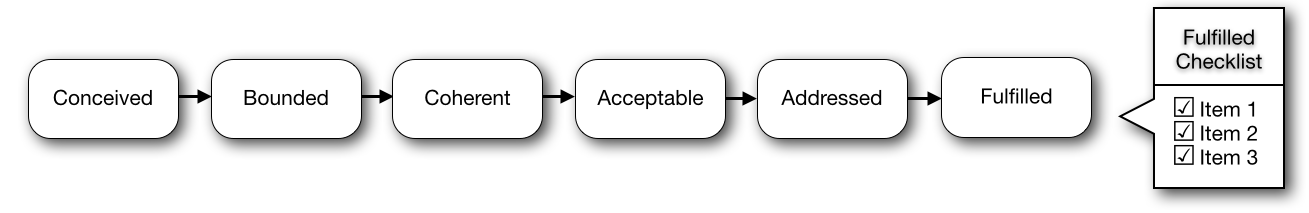
\includegraphics[width=5.4in]{kernel_images/StateMachineRequirements}}
\caption{Kernel's linear state machine for Requirements alpha}\vspace*{-6pt}\label{StateMachine}
\end{figure}

When the SEMAT community created the Essence kernel, they relied upon human experience and judgment to select the alphas, states, and checklists. Essence is not grounded by empirical data. There might be other possible groupings of checklist items that are more effective which we might not normally consider because they do not match our preconceived notions of structure and order.

We leverage empirical data to both evaluate possible candidate kernels. During the Spring 2014 and Summer 2014 semesters, graduate software engineering students at Carnegie Mellon University in Silicon Valley recorded their progress during their software engineering practicum course. Each team recorded which checklist items the team accomplished during their weekly Essence Reflection meetings. \cite{EASE2014}

% \textbf{Goal 2:} Using a genetic algorithm, make small incremental improvements to the Essence kernel.

\section{Experiment Planning}
\subsection{Optimization Goal}
\label{Optimization Application}
The goal is the optimization of candidate kernels using a fitness function based on empirical data in order to create an alternative Essence kernel. This is not a real time problem such as stock market analysis requiring highly performing input to output calculations.

% The optimization problem of \textbf{Goal 1} means finding a single better candidate grounded in the data as described in Table~\ref{Goal of Program}. 

\subsection{Genotype Data Structure}

Creating a candidate kernel requires a permutation of the kernel's 148 checklist items into states in different alphas, optimized by a fitness function.

% \begin{table}[h]
% \caption{Genetic Algorithm's Purpose}
% \label{Goal of Program}
% \label{Goal}
% \centering
% \begin{tabular}{|p{0.80in}|p{2.30in}|}
% \hline
% {Goal:}  & {The optimization of} \\ \hline
% {Input:} & {candidate kernels}  \\ \hline
% {Model:} & {using a fitness function based on empirical data} \\ \hline
% {Output:} & {in order to create the “best” kernel} \\ \hline
% \end{tabular}
% \end{table}

% We first determine the data structure for the genetic algorithm. Since each alpha is a linear state machine, a simple representation for an alpha is: 
% \begin{verbatim}
% alpha: [state1, state2, ... state6] 
% \end{verbatim}

% Since each state is a collection of checklist items, and each checklist item is a unique identifier, an alpha becomes:

% \begin{verbatim}
% alpha: [{5,8,11}, {6}, ... {7,9,10,52}]
% \end{verbatim}

% A kernel of many alphas can thus be represented by:

% \begin{verbatim}
% kernel = {
%   alpha_1: [{5,8,11}, {6}, ... {7,9,10,52}],
%   alpha_2: [{42,57,58}, {32,35}],
%   alpha_3: [...]
%   ...
% }
% \end{verbatim}

We first determine the data structure for the genetic algorithm. Since each alpha is a linear state machine and each state is a collection of checklist items, and each checklist item is a unique identifier, a kernel of many alphas can be represented by:

\begin{verbatim}
kernel = {
  alpha_1: [{5,8,11}, {6}, ... {7,9,10,52}],
  alpha_2: [{42,57,58}, {32,35}],
  alpha_3: [...]
  ...
}
\end{verbatim}

This data structure serves as the genetic algorithm's genotype. As the genetic algorithm modifies this data structure, it explores the search space of possible candidate kernels. In genetic algorithm terminology, the genotype represents the chromosomes to be altered whereas the phenotype represents the real world manifestation of those traits such as eye or hair color. The data structure conveniently represents the kernel or phenotype as it is easy to describe the kernel from the data structure.\cite{Eiben2003} 

\subsection{Evolutionary Algorithm}
\label{Evolutionary Algorithm}

Given the genotype representation, we created a genetic program as described in Table~\ref{TechnicalSummary} that has mutation operators uniquely tailored to the representation.

Genetic algorithms typically initialize a population of random candidate solutions (also known as individuals). In this case each member of the population is a candidate kernel. The code initializes the kernel with a random number of states per alpha and then distributes the 148 checklist items randomly to the states. The population size initialized to 40 members.

Once initialized, genetic algorithms typically run for a number of generations until either the population stabilizes or a fixed number of generations have passed. During each generation, a genetic algorithm copies and alters each member of the population to create offspring. Our genetic program utilized deterministic parent selection where every member of the population would create one offspring. Given the uniqueness of the data structure, instead of typical mutation and crossover operators, we created specific operators to randomly alter the distribution of checklist items. For each member of the population, a random number determined which mutation operator would be used. The weights are arbitrary and future research can determine the ideal frequency ratios for the operators. 

\begin{itemize}
\item ``Move checklist item" operator randomly selects a checklist item and moves it to a different state. If the new state has more than eight checklist items, the code automatically splits that state into two states using the ``split state" operator. The genetic program choose this operator 80\% of the time.
\item ``Split state" operator randomly selects a state and subdivides it by creating a new subsequent state and moves half of the checklist items to the new state. The genetic program choose this operator 10\% of the time.
\item ``Delete state" operator randomly deletes a state by moving all of its checklist items to other states. The genetic program choose this operator 10\% of the time.
\end{itemize}

Once all of the offspring are created, the code implements ``comma survivor selection" by adding each offspring to the population pool, sorting the parents and offspring together, and retaining only the top 50\% of the combined population. This is also known as elitism as the population can only increase its fitness scores. The code would terminate once 500 generations had been created.

% \begin{table}[h]
% \caption{Evolutionary Algorithm Technical Summary}
% \label{TechnicalSummary}
% \centering
% \begin{tabular}{|p{1.70in}|p{4.30in}|}
% \hline
% {Type}  & {Genetic Programming} \\ \hline
% {Representation} & {Collection of states which are a collection of checklist items}  \\ \hline
% {Crossover and} & {1) move checklist item (to another state) (80\%), } \\
% {Mutation} & {2) split state into two states (10\%), } \\ 
% {} & {3) delete state (by randomly moving its checklist items) (10\%) } \\ \hline
% {Parent selection} & {Deterministic} \\ \hline
% {Survivor selection}  & {Comma} \\ \hline
% {Population size}  & {40} \\ \hline
% {Termination \mbox{condition}} & {500 generations} \\ \hline
% \end{tabular}
% \end{table}

\begin{table}[h]
\caption{Evolutionary Algorithm Technical Summary}
\label{TechnicalSummary}
\centering
\begin{tabular}{p{1.70in}p{4.30in}}
\hline
{Type}  & {Genetic Programming} \\ 
{Representation} & {Collection of states which are a collection of checklist items}  \\ 
{Crossover and Mutation} & {1) move checklist item (to another state) (80\%), } \\
{} & {2) split state into two states (10\%), } \\ 
{} & {3) delete state (by randomly moving its checklist items) (10\%) } \\ 
{Parent selection} & {Deterministic} \\ 
{Survivor selection}  & {Comma} \\ 
{Population size}  & {40} \\ 
{Termination \mbox{condition}} & {500 generations} \\ 
\hline
\end{tabular}
\end{table}

\section{Fitness Functions}

Since there is no prior work describing how to evaluate candidate kernels, we created two fitness functions for the purpose of exploring candidate evaluations called Partial Ordering and Completion fitness functions. 
\subsection{Partial Ordering Fitness Function}
When considering a given week's worth of data for a team, the Partial Ordering fitness function compares the checklist items that were done during that week with the ones that were done before and after. The fitness function rewards candidates that match the partial ordering of the empirical data. During each week, the fitness function pairwise considers each accomplished checklist with all of its predecessors and successors. 
% Do not delete, include in phd.
% \subsubsection{Rationale}
% While we know that these checklist items were accomplished during the same week, we do not know if accomplishing the checklist items are correlated. It could be the case that many different events happened during the week to cause different checklist items to be accomplished. Consider the different cases about what can happen with the Essence States. 

% Case 1) While the team is making progress on their projects, it could be the case that nothing changes from one week to the next and their Essence States stay the same. This tends to happen during the Construction phase of the project as the team progresses through their backlog. \cite{ICSE2014}

% Case 2) A single event happened and caused a state transition. This event causes all changes in checklists. The ideal Essence kernel would perfectly model this transition. As a hypothetical example, a meeting with the client to identify stakeholder groups and representatives for each group would cause 5 and 8 to be accomplished in Week 1 of Figure ~\ref{delta}.

% Case 3) Multiple events happened and they caused multiple transitions. In Week 2 of Figure ~\ref{delta}, one event, E1 may cause checklist items 6 and 11 to be checked and event E2 may cause checklist items 7 and 20 to be checked. The empirical data we does not inform us about E1 and E2; all we see is that {6, 7, 11, 20} become checked. 

% We can not distinguish between Case 2 and Case 3 from the data. When the Essence States do change, one or many events that happened during the previous week may be responsible. While we do not know the relationship with the data during a week, we do know the relationship with the data from week to week.

% For a given week \textit{i}, we do know that there is a partial ordering between the data before week \textit{i}, week \textit{i}, and the data after week \textit{i}. Consider Week 3 of Figure ~\ref{delta}, we know that all the checklist items that happened before {1, 10, 21} and all the checklist items that happened after {1, 10, 21}. We can reward candidate solutions that respect this partial ordering.

\subsubsection{Partial Ordering Example}

During weekly Essence Reflection meetings, the team records its progress across every alpha by reviewing checklist items ~\cite{ICSE2014}. Figure ~\ref{history} shows the progression of a hypothetical team through the checklists.

\begin{figure}[!htb]
\begin{verbatim}
Week 1: {5, 8}
Week 2: {6, 7, 11, 20} 
Week 3: {1, 10, 21} 
...
\end{verbatim}
 \caption{History of Team's Progress from Essence Reflection Meetings}
 \label{history}
\end{figure}

Consider the naive candidate solution in Figure ~\ref{sequential_candidate} which is a sequential listing of all checklists. This candidate suggests that a project would accomplish each checklist item, one at a time.

\begin{figure}[!htb]
\begin{verbatim}
kernel = {
  alpha: [{1}, {2}, {3}, {4}, {5}, {6}, 
          {7}, {8}...{148}]
}
\end{verbatim}
 \caption{Sequential Candidate}
 \label{sequential_candidate}
\end{figure}

Partial Ordering gives a point to the candidate for correctly matching the time sequence of the data. For illustrative purposes, consider the evaluation of Week 2 using the data in Figure ~\ref{history}. The team accomplished the checklist items in Week 1 before accomplishing the checklist items in Week 2. Thus Partial Ordering considers if the candidate has the checklist items for Week 1 occurring before Week 2. The fitness function checks the candidate to see if 5 and 8 precede 6, 7, 11, and 20. Then, Partial Ordering compares if the candidate has the checklist items for Week 2 occurring prior to Week 3. The fitness function examines if 6, 7, 11, and 20 precede 1, 20, 21. While comparing the empirical data against the candidate solution, the candidate represents some, but not all of this behavior. Partial Ordering follows this procedure for the all weeks of the project for every team in the empirical data set. %Figure ~\ref{evaluation_example} describes each step.
%Whenever the model correctly represents the empirical data, it earns a point. Candidate solutions that score the most points best represent the empirical data.

% \begin{figure}[!htb]
% \begin{verbatim}
% # Compare earlier checklists (5, 8)     # Compare later checklists (1, 10, 21)
% # against current week                  # against current week

% 5 before? 6 => yes                      6 before? 1 => no
% 8 before? 6 => no                       6 before? 10 => yes
%                                         6 before? 21 => yes
% 5 before? 7 => yes                  
% 8 before? 7 => no                       7 before? 1 => no
%                                         7 before? 10 => yes
% 5 before? 11 => yes                     7 before? 21 => yes
% 8 before? 11 => yes                     
%                                         11 before? 1 => no 
% 5 before? 20 => yes                     11 before? 10 => yes
% 8 before? 20 => yes                     11 before? 21 => yes
                                        
%                                         20 before? 1 => no
%                                         20 before? 10 => yes
%                                         20 before? 21 => yes
% Score: 14 / 20 for week 2
% \end{verbatim}
%  \caption{Partial Ordering Evaluation Example for Week 2}
%  \label{evaluation_example}
% \end{figure}

% \subsubsection{Psuedocode}
% Figure \ref{psuedocode} shows the psuedocode for evaluating a candidate solution against the empirical data. The running time of the algorithm is O(t * m * k * k) where
% t = number of teams,
% m = number of meetings with each team, and
% k = average number of checklists per meeting.

% \begin{figure*}[ht]
% \begin{verbatim}
% evaluate(candidateSolution)
%   for each team in empirical data
%     earlierChecklists is empty
%     laterChecklists is team's checklists
%     for each meeting in team'sData
%       for each checklist in meeting
%         scoreBeforeOrEquals(checklist, laterChecklists)
%         scoreEqualsOrAfter(checklist, earlierChecklists)
%         add checklist to earlierChecklists 
%         remove checklist from laterChecklists
% \end{verbatim}
%  \caption{Psuedocode for Partial Order Fitness Function}
%  \label{psuedocode}
% \end{figure*}

\subsection{Completion Fitness Function}
The Completion fitness function assigns points when checklists are done in the right order. Just like the Essence kernel requires all checklist items to be accomplished before the states is achieved, the Completion fitness only awards points when all checklists are done on a card before progressing to future cards in the same alpha. The Completeness fitness function measures how perfectly the candidate matches the empirical data. 

% \begin{lstlisting}[language=C,frame=single,caption=Psuedocode for Completion Fitness Function,label=psuedocodeCompletion]
% For each team’s data, the individual scores 1 point for each transition of checklist items they correctly represent. If a team does not achieve a state card, future checklists in that alpha do not count
% \end{lstlisting}

In practice, the Completion fitness function acts as a strict professor rigorously grading assignments, never giving partial credit for mostly right answers. As soon as something is wrong in the state sequence, it is over for scoring points. The only way for a candidate kernel to have a high score is to correctly represent the initial states of an alpha.

%Consider the situation where a genetic algorithm randomly puts a checklist item that happens at the end of the project on the first card. Since the only way to score points for the second and subsequent cards is to accomplish everything on the first card, the candidate kernel will \textit{only} score points for the checklist items on the first card. If there are k checklist items on the first card, it will score k-1 points.

In retrospect, completion is not an ideal fitness function. Since genetic algorithms thrive in environments of partial credit \cite{Eiben2003}. Thus this paper will focus the discussion on the Partial Ordering fitness function.

\section{Understanding the kernel search space}
% In order to optimize the initial conditions of the genetic algorithm, we first need to understand how the fitness function responds to different parameters including:

% \begin{itemize}
% \item How does the number of alphas affect the fitness scores?
% \item How do the mutation operators affect the fitness scores?
% % \item How does the algorithm utilize states?
% \end{itemize}

\subsection{How does the number of alphas affect the fitness scores?}
We conducted a series of experimental runs by setting the initial population so that all candidates start with the same number of alphas. We inspected the population after the algorithm has run for a number of generations to see how the number of alphas affects the fitness score. Note that the current set of operators can not alter the number of alphas.

% \begin{table}[h]
% \caption{Number of Alphas and Fitness Scores for Partial Ordering}
% \label{NumberOfAlphas}
% \centering
% \begin{tabular}{|l|r|r|}
% \hline
% Number of Alphas & \multicolumn{2}{c|}{Fitness Score} \\ \hline
%                  & Gen 0            & Gen 200            \\ \hline
% { 1 } & { 58606 } & { 78530 } \\ \hline
% { 2 } & { 30540 } & { 70452 } \\ \hline
% { 3 } & { 20842 } & { 68344 } \\ \hline
% { 4 } & { 16146 } & { 41040 } \\ \hline
% { 5 } & { 13150 } & { 43636 } \\ \hline
% { 6 } & { 11718 } & { 49408 } \\ \hline
% { 7 } & { 10254 } & { 34990 } \\ \hline
% { 8 } & {  9010 } & { 31560 } \\ \hline
% \end{tabular}
% \end{table}

\begin{table}[h]
\caption{Number of Alphas and Fitness Scores for Partial Ordering}
\label{NumberOfAlphas}
\begin{tabular}{lrr}
\hline
Number of Alphas & \multicolumn{2}{c}{Fitness Score}     \\
                 & Gen 0            & Gen 200            \\ \hline
{ 1 } & { 58606 } & { 78530 } \\ 
{ 2 } & { 30540 } & { 70452 } \\ 
{ 3 } & { 20842 } & { 68344 } \\ 
{ 4 } & { 16146 } & { 41040 } \\ 
{ 5 } & { 13150 } & { 43636 } \\ 
{ 6 } & { 11718 } & { 49408 } \\ 
{ 7 } & { 10254 } & { 34990 } \\ 
{ 8 } & {  9010 } & { 31560 } \\ 
\hline
\end{tabular}
\end{table}

The Partial Ordering fitness function prefers low number of alphas. Table ~\ref{NumberOfAlphas} shows for each alpha, the best individual's fitness score for the initial population, and the population after 200 generations. In the initial random populations we see that one alpha is the highest scoring run.

When initialized to a larger number of alphas, the genetic algorithm will discover that not using some of the alphas is advantageous. Starting with eight populated alphas, after 200 generations, three of the eight alphas are empty, and two are very sparse as seen in Table ~\ref{PartialOrderingPrefersLessAlphas}.

% \begin{table*}
% \caption{Number of Checklist Items Per State Per Alpha \\ Candidates Starting with Eight Alphas Evolve To Use Less Alphas with Partial Ordering}
% \label{PartialOrderingPrefersLessAlphas}
% \centering
% \begin{tabular}{|l|l|l|l|l|l|l|l|l|l|l|l|l|l|l|l|}
% \hline
%  & \multicolumn{15}{l|}{state} \\ \hline
%  & 1  & 2  & 3  & 4  & 5  & 6  & 7  & 8  & 9  & 10  & 11  & 12  & 13  & 14  & 15 \\ \hline
% alpha 1 &   &   &   &   &   &   &   &   &   &   &   &   &   &   &   \\ \hline
% alpha 2 & 5 & 1 &   &   &   &   &   &   &   &   &   &   &   &   &   \\ \hline
% alpha 3 &   &   &   &   &   &   &   &   &   &   &   &   &   &   &   \\ \hline
% alpha 4 & 1 & 1 & 1 &   &   &   &   &   &   &   &   &   &   &   &   \\ \hline
% alpha 5 & 5 & 8 & 4 & 3 & 7 & 7 & 7 & 4 & 5 & 2 & 2 &   &   &   &   \\ \hline
% alpha 6 & 5 & 6 & 4 & 4 & 6 & 7 & 6 & 7 & 6 & 7 & 8 & 4 & 5 & 8 & 8 \\ \hline
% alpha 7 & 2 & 6 & 7 & 5 & 4 & 2 &   &   &   &   &   &   &   &   &   \\ \hline
% alpha 8 &   &   &   &   &   &   &   &   &   &   &   &   &   &   &   \\ \hline
% \end{tabular}
% \end{table*}

\begin{table*}
\caption{Number of Checklist Items Per State Per Alpha}
\label{PartialOrderingPrefersLessAlphas}
\begin{tabular}{llllllllllllllll}
\hline
 & \multicolumn{15}{l}{state} \\ 
 & 1  & 2  & 3  & 4  & 5  & 6  & 7  & 8  & 9  & 10  & 11  & 12  & 13  & 14  & 15 \\ \hline
alpha 1 &   &   &   &   &   &   &   &   &   &   &   &   &   &   &   \\ 
alpha 2 & 5 & 1 &   &   &   &   &   &   &   &   &   &   &   &   &   \\ 
alpha 3 &   &   &   &   &   &   &   &   &   &   &   &   &   &   &   \\ 
alpha 4 & 1 & 1 & 1 &   &   &   &   &   &   &   &   &   &   &   &   \\ 
alpha 5 & 5 & 8 & 4 & 3 & 7 & 7 & 7 & 4 & 5 & 2 & 2 &   &   &   &   \\ 
alpha 6 & 5 & 6 & 4 & 4 & 6 & 7 & 6 & 7 & 6 & 7 & 8 & 4 & 5 & 8 & 8 \\ 
alpha 7 & 2 & 6 & 7 & 5 & 4 & 2 &   &   &   &   &   &   &   &   &   \\ 
alpha 8 &   &   &   &   &   &   &   &   &   &   &   &   &   &   &   \\ \hline
\end{tabular}
\end{table*}


For the Partial Ordering fitness function, initializing the population to a single alpha results in the most fit candidates. 

Given this result, the genetic algorithm challenges us to consider creating an Essence kernel with a single alpha. The original kernel is arranged into seven alphas based upon human constructs of software systems, yet this might not be ideal for Essence Reflection meetings. During Essence Reflection meetings, a team considers possible next goals to accomplish. With seven alphas, team members must consider a significant number of checklist items. With a single alpha, a team could simply consider a limited set of next possible goals. Imagine a team meeting with the perfect oracle, once describing their current state, the oracle could suggest several possible goals informed by the collective experience of previous teams. Creating such an oracle may require a fundamental shift in the data representation of the Essence kernel.

\subsection{How do the mutation operators affect the fitness scores?}
As another experiment, we ran 40 runs for five generations to see the impact of each operator on fitness score. By limiting to early generations, there is still plenty of opportunity for large changes in fitness. During each run, the program records the fitness differential before and after applying an operator. Figure ~\ref{OperatorsPartialOrdering} plots the distribution of fitness deltas per mutation operator.

\begin{figure}[ht]\vspace*{4pt}
\centerline{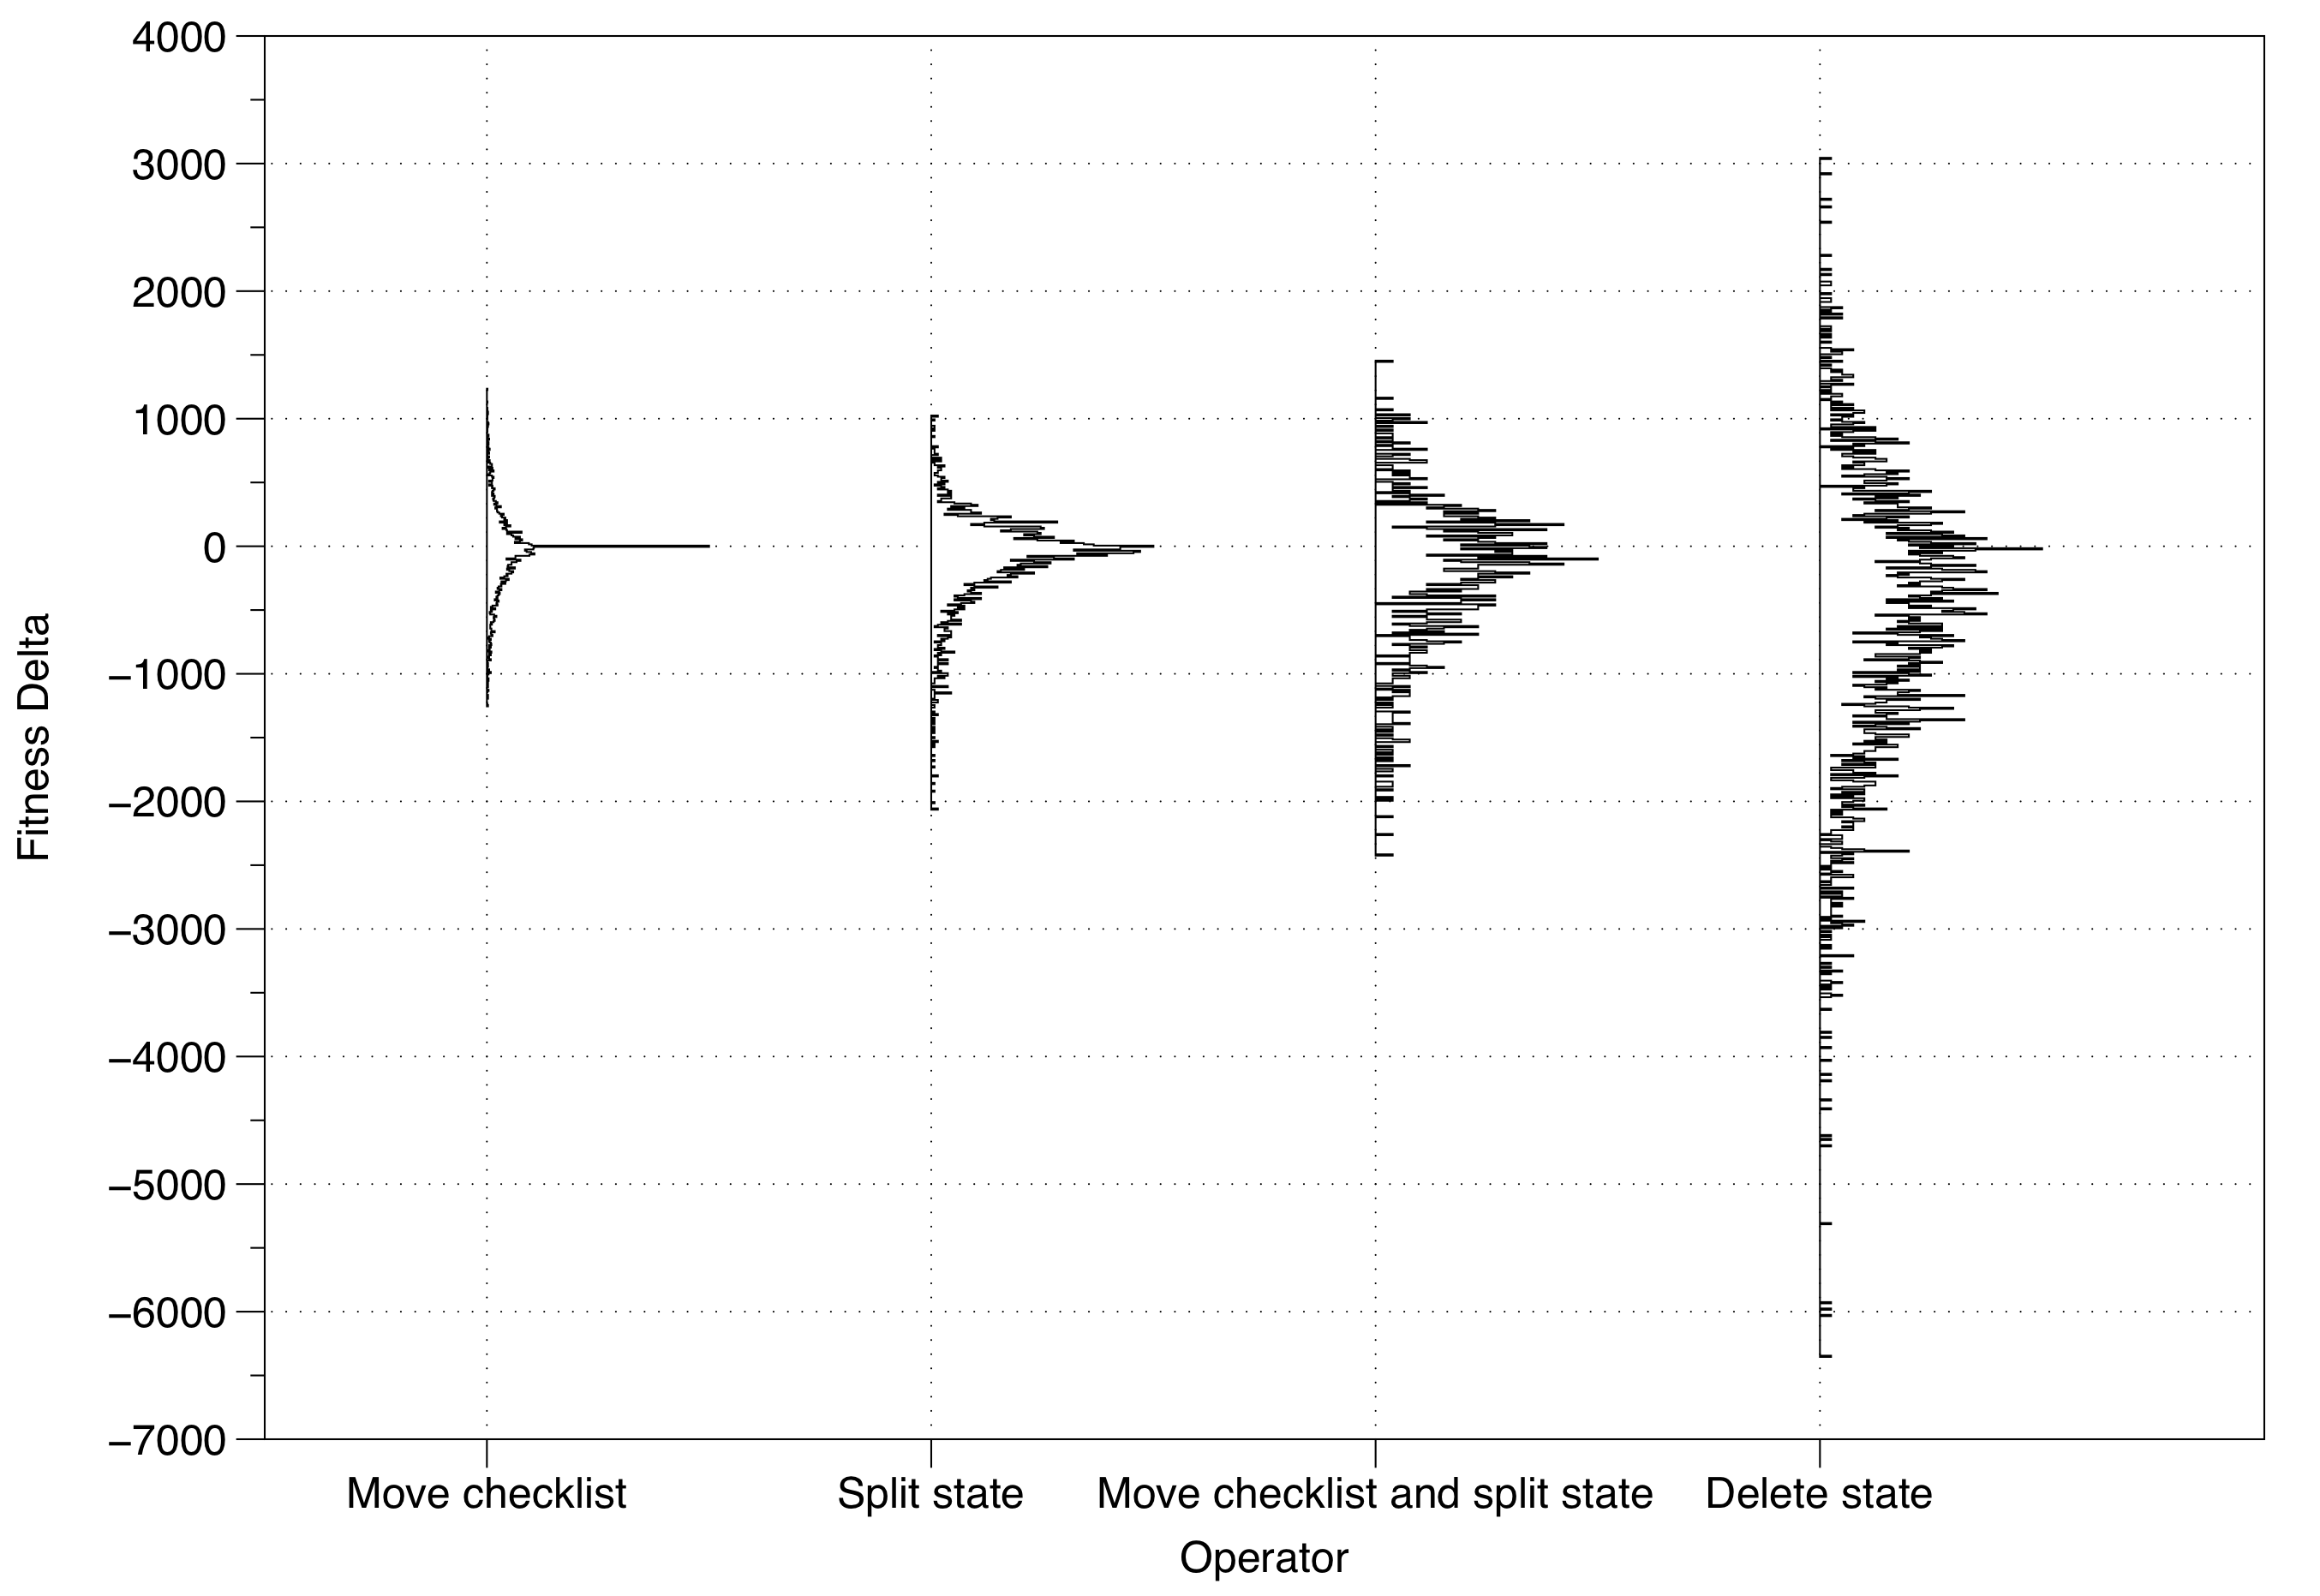
\includegraphics[width=4.0in]{images/operator_analysis_partial_order_first_5_gens}}
\caption{Mutation Operators Effect on Fitness Scores for Partial Ordering}\vspace*{-6pt}
\label{OperatorsPartialOrdering}
\end{figure}

\begin{itemize}
  \item ``move checklist" typically has the smallest impact on the fitness scores. Most of the distribution is tightly centered around zero. This operator is great for fine tuning a well established structure. 
  \item ``move checklist and split state" occurs when ``move checklist" adds a  checklist to a state that already has eight, causing an automatic split to happen. The distribution is similar to ``split state."
  \item ``split state" is a more ``destructive" operator to the data structure and has a wider range of impact than ``move checklist"
  \item ``delete state" causes the most change to the data structure and has the largest impact on fitness scores. 
\end{itemize}

The mean of all of these mutation operators is slightly negative. As with most genetic algorithms, applying any operator can cause a fitness score decrease and the offspring will eventually be discarded when the population surpasses it.

% \subsection{How does the algorithm utilize states?}

% Partial Ordering maintains a consistent number of states over time. Figure ~\ref{NumberOfStatesPartialOrdering} illustrates how a population utilizes the number of states when constrained to four alphas. The randomly created initial population ranges from 23 to 38 states and evolves to use roughly 25 to 30 states through out its generations. A stable number of states, as opposed to an infinitely growing number of states, is a desirable property for a fitness function. 

% \begin{figure}[ht]\vspace*{4pt}
% \centerline{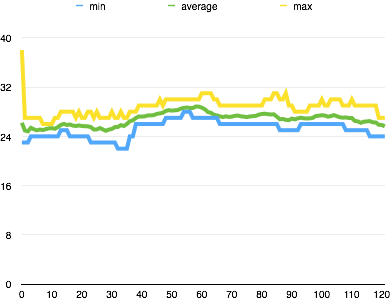
\includegraphics[scale=0.6]{images/number_of_states_partial_ordering}}
% \caption{Number of States Fitness Analysis for Partial Ordering}\vspace*{-6pt}
% \label{NumberOfStatesPartialOrdering}
% \end{figure}

\section{Best Generated Candidate Kernel}

Given that the Partial Ordering fitness function prefers smaller number of alphas, the best scoring candidates emerge quickly when starting with only a single alpha. Figure ~\ref{BestResultsPartialOrdering} shows the best, average, and worst fitness scores over 500 generations for 40 runs. (These 40 runs completed in 12.65 hours.) The graph also plots the fitness score of the original kernel.

The original kernel scores 13,372. The best generated kernel scores 85,122. For the Partial Ordering fitness function, the genetic algorithm had little difficulty in finding random solutions that score higher than the original kernel. The original kernel is optimized for human understanding and places 148 checklist items into logical sequences around themed alphas where as the candidate kernels are optimized around how teams actually flow through the checklist items.

\begin{figure*}[ht]\vspace*{4pt}
\centerline{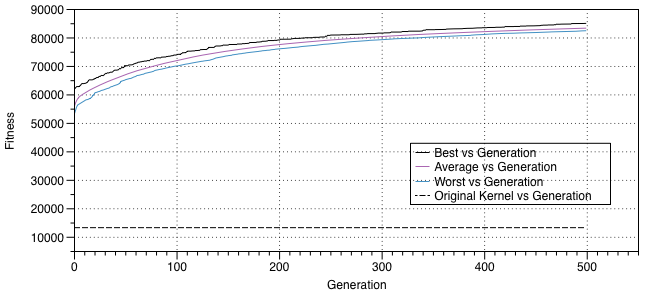
\includegraphics[width=6.25in]{images/best_results_partial_ordering_500gens_40runs}}
\caption{Fitness Scores using Partial Ordering}\vspace*{-6pt}
\label{BestResultsPartialOrdering}
\end{figure*}

Table ~\ref{BestResults} shows the beginning two states for the final candidate which is a single alpha with 30 sequential states. The states contain a mixture of checklist items from different alphas. The candidate interweaves alphas into one flow based upon how teams accomplished the checklist items in practice. 

The generated kernel revealed that several checklists items that occur later in the original kernel often happen earlier on real projects. For example, the generated kernel places ``Team values stakeholders representatives' input" in the second state. Likewise, several checklist items that occur early in the original kernel often happen later on real projects. For example, the generated kernel places ``Defect levels are acceptable" in the second to last state. In future work, more analysis can be done with sufficient number of teams.

% \begin{table}[h]
% \caption{Highest Scoring Essence Kernel Generated By Genetic Algorithm}
% \label{BestResults}
% \centering
% \begin{tabular}{|p{0.50in}|p{2.80in}|p{1.00in}|p{1.40in}|}
% \hline
% State & Checklist & Original \mbox{Alpha} & Original State \\ \hline
% State 1 & Stakeholders wish to make an investment in better understanding potential value & Opportunity & 1. Identified \\ \hline
% State 1 & User types are identified & Requirements & 1. Conceived \\ \hline
% State 1 & Team agrees on relevant stakeholder groups to be represented & Stakeholders & 1. Recognized \\ \hline
% State 1 & Representatives respect team's way of working  & Stakeholders & 2. Represented \\ \hline
% State 2 & An idea for a software solution is identified & Opportunity & 1. Identified \\ \hline
% State 2 & Funding model is clear & Work & 1. Initiated \\ \hline
% State 2 & Stakeholder representatives agree to take on responsibilities & Stakeholders & 2. Represented \\  \hline
% State 2 & Team values stakeholder representatives' input & Stakeholders & 4. In Agreement \\ \hline
% State 2 & Opportunity addresses problem and stakeholder needs & Opportunity & 2. Solution Needed \\ \hline
% ... &  & \\ \hline
% \end{tabular}
% \end{table}

\begin{table}[h]
\caption{Highest Scoring Essence Kernel Generated By Genetic Algorithm}
\label{BestResults}
\centering
\begin{tabular}{p{0.50in}p{2.80in}p{1.00in}p{1.40in}}
\hline
State & Checklist & Original \mbox{Alpha} & Original State \\ \hline
State 1 & Stakeholders wish to make an investment in better understanding potential value & Opportunity & 1. Identified \\ 
State 1 & User types are identified & Requirements & 1. Conceived \\ 
State 1 & Team agrees on relevant stakeholder groups to be represented & Stakeholders & 1. Recognized \\ 
State 1 & Representatives respect team's way of working  & Stakeholders & 2. Represented \\
State 2 & An idea for a software solution is identified & Opportunity & 1. Identified \\ 
State 2 & Funding model is clear & Work & 1. Initiated \\ 
State 2 & Stakeholder representatives agree to take on responsibilities & Stakeholders & 2. Represented \\ 
State 2 & Team values stakeholder representatives' input & Stakeholders & 4. In Agreement \\
State 2 & Opportunity addresses problem and stakeholder needs & Opportunity & 2. Solution Needed \\
... &  & \\ \hline
\end{tabular}
\end{table}

% \section{Optimizing the Original Kernel}

% With the genetic algorithm code, we are able to optimize the existing kernel.

% To accomplish this, we utilized the following greedy algorithm: 
% First, iterate over the checklists and find the checklist item that would increase the fitness score the most if it was either moved forward or later. Second, move it. Third, repeat until there are no improvements in fitness score.

% The starting fitness score is 13,372 and it improves to 13,490 by moving 22 checklist items. In examining the final optimized kernel, several states can be combined. The \textbf{Stakeholder}'s \textit{Recognized} and \textit{Represented} states can be combined (Figure \ref{StakeholdersRecognized}). The \textbf{Team}'s \textit{Concluded} and \textit{Closed} states can be combined (Figure \ref{TeamConcluded}). From the empirical data, there is no clear distinction between these states as the states happen concurrently in practice.

% \begin{figure}[ht]
% 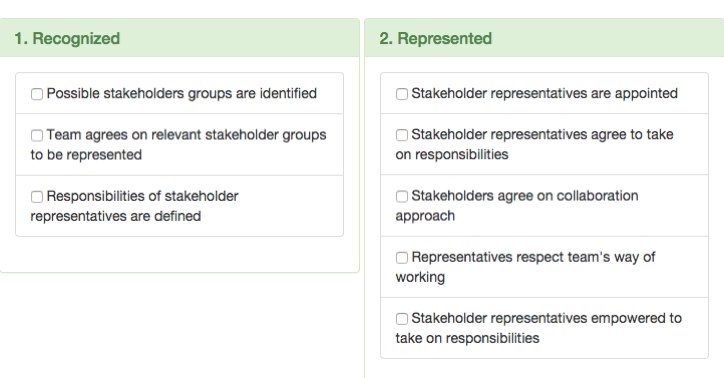
\includegraphics[scale=0.33]{kernel_images/stakeholders_1_2}
% \caption{Stakeholder's Recongized and Represented States Could be Combined}
% \label{StakeholdersRecognized}
% \end{figure}

% \begin{figure}[ht]
% 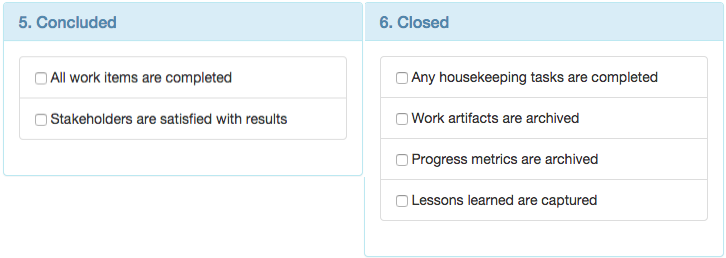
\includegraphics[scale=0.33]{kernel_images/team_5_6}
% \caption{Team's Concluded and Closed States Could be Combined}
% \label{TeamConcluded}
% \end{figure}

% The algorithm also revealed that several checklist items listed early in the original kernel often happen later on a real project:

% \begin{itemize}
% \item{\textbf{Opportunity}'s Desired outcomes are clear}
% \item{\textbf{Opportunity}'s Success criteria are clear}
% \item{\textbf{Software System}'s Selected architecture addresses key technical risks}
% \item{\textbf{Software System}'s Defect levels are acceptable}
% \end{itemize}

% If this is consistent with data from additional teams, then this suggests that these checklist items should be moved to a later state. 

\section{Threats to Validity}

\underline{Generalizability across situations}: the collected data is from faculty facilitating Essence Reflection meetings \cite{EASE2014} with masters of software engineering teams during their final practicum project at Carnegie Mellon University in Silicon Valley. This empirical data, and thus the results, may not represent teams in industry nor teams at other universities. Replicating the results from \cite{ICSE2014} would mitigate this threat.

\underline{Limited amount of empirical data}: the collected data is from five teams collecting data every week during the duration of a fifteen week semester. As a result, the generated solutions might be over-optimized to the empirical data. Collecting more data will diminish this threat. The purpose of this work is to show initial results in applying genetic algorithms for fitting possible candidate kernels to empirical data, not to recommend a replacement for the original Essence kernel. 

\section{Conclusions and Future Work}

This paper describes how a genetic algorithm created random kernels using two different fitness functions. The candidate kernels have the same fundamental structure as the original Essence kernel: a collection of linear state machines called alphas with each state having a set of checklist items. 

We analyzed the genetic algorithm's search space. The Partial Ordering fitness function prefers smaller number of alphas and typically relies upon a stable number of states. Applying the ``delete state" mutation operator has the widest positive and negative effect on the resultant fitness score whereas the ``move checklist" and ``split state" have a narrower effect on fitness scores. 

% Since generated candidates can not represent all empirical data perfectly, an ideal fitness function rewards candidates that fit the data well. The Partial Ordering fitness function has this characteristic. With enough empirical data, we expect there to be common patterns amongst teams. Ideal fitness function rewards models that represent common flows through the Essence states.

The best generated random kernel scores higher than the original Essence kernel. 

Optimizations to the original Essence kernel are possible. Using the same code base, a greedy optimization algorithm altered the original Essence kernel and revealed that several states could be combined and several checklist items could move to better represent the empirical data collected so far.

As for next steps, collecting more empirical data will yield more reliable results and better insights. %Future research includes considering an ALPS strategy \cite{ALPS} of age-based population pools. 
Given the mutation operator analysis on fitness, one strategy to consider is starting with operations that have large structural changes in younger populations, and then later optimizing checklists within a given structure. Additional research can experiment with how population size and weights of operators affect the genetic algorithm's performance. %Additional experiments could consider altering the fitness function to have other desirable kernel properties such as limiting number of states or requiring a minimum number of alphas to be used.

In conclusion, genetic algorithms explore the kernel search space through random mutations. Given the human desire for order, the computer can consider solutions that people might immediately dismiss as not meeting certain aesthetic considerations. By considering these unusual solutions, the computer can further optimize the solution to achieve higher scoring candidate kernels. 


% Show this to Cecile

% \begin{table}[h]
% \caption{Starting State for Genetic Algorithms Like to Cheat}
% \label{CompletionCheatsInitial}
% \centering
% \begin{tabular}{|l|l|l|l|l|l|l|}
% \hline
% alpha 1 & 6 & 4 & 2 & 3 & 4 & 5 \\ \hline
% alpha 2 & 5 & 4 & 3 & 5 & 3 & 4 \\ \hline
% alpha 3 & 5 & 3 & 4 & 4 & 1 & 4 \\ \hline
% alpha 4 & 6 & 3 & 5 & 7 & 3 & 4 \\ \hline
% alpha 5 & 4 & 9 & 5 & 2 & 1 & 3 \\ \hline
% alpha 6 & 2 & 6 & 7 & 5 & 4 & 2 \\ \hline
% \end{tabular}
% \end{table}

% \begin{table}[h]
% \caption{Final State for Genetic Algorithms Like to Cheat}
% \label{CompletionCheatsFinal}
% \centering
% \begin{tabular}{|l|l|}
% \hline
% alpha 1 & 34 \\ \hline
% alpha 2 & 12 \\ \hline
% alpha 3 & 2  \\ \hline
% alpha 4 & 31 \\ \hline
% alpha 5 & 35 \\ \hline
% alpha 6 & 33 \\ \hline
% \end{tabular}
% \end{table}



% \begin{figure}[ht]
% 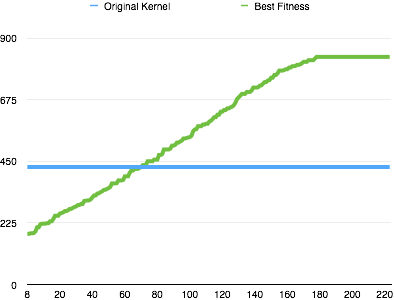
\includegraphics[scale=0.6]{images/initial_results_completion}
% \caption{Initial Results for Completion}\label{InitialResultsCompletion}
% \end{figure}

% \begin{figure}[ht]
% 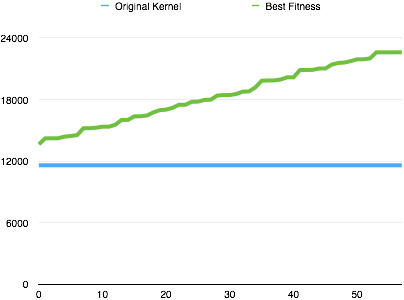
\includegraphics[scale=0.6]{images/initial_results_partial_ordering}
% \caption{Initial Results for PartialOrdering}\label{InitialResultsPartialOrdering}
% \end{figure}

% \begin{figure}[ht]
% 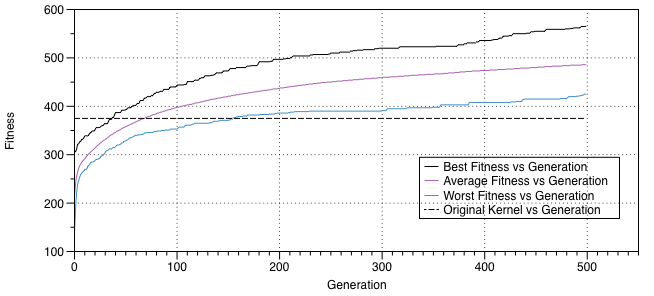
\includegraphics[scale=0.37]{images/best_results_completion_500gens_40runs}
% \caption{Best Results for Completion}\label{BestResultsCompletion}
% \end{figure}

% \begin{figure}[ht]
% 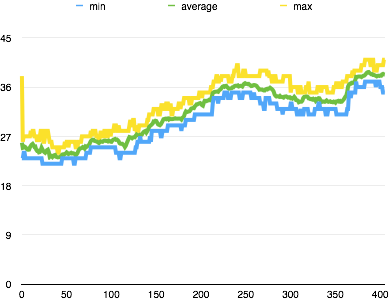
\includegraphics[scale=0.6]{images/number_of_states_completion}
% \caption{Number of States Fitness Analysis for Completion}\label{NumberOfStatesCompletion}
% \end{figure}

% \begin{figure}[ht]
% 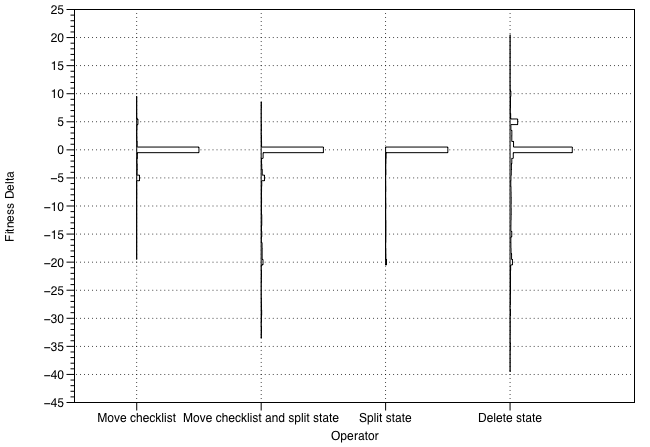
\includegraphics[scale=0.37]{images/operator_analysis_completion_first_5_gens}
% \caption{Mutation Operators Affect on Fitness Scores for Completion}\label{OperatorsCompletion}
% \end{figure}


%% References
%%
%% Following citation commands can be used in the body text:
%% Usage of \cite is as follows:
%%   \cite{key}         ==>>  [#]
%%   \cite[chap. 2]{key} ==>> [#, chap. 2]
%%

%% References with bibTeX database:

% \bibliographystyle{elsarticle-num}
% \bibliographystyle{elsarticle-harv}
% \bibliographystyle{elsarticle-num-names}
% \bibliographystyle{model1a-num-names}
% \bibliographystyle{model1b-num-names}
% \bibliographystyle{model1c-num-names}
% \bibliographystyle{model1-num-names}
% \bibliographystyle{model2-names}
\bibliographystyle{model3a-num-names}
% \bibliographystyle{model3-num-names}
% \bibliographystyle{model4-names}
% \bibliographystyle{model5-names}
% \bibliographystyle{model6-num-names}

\bibliography{bibliography}

\end{document}

%%
%% End of file `elsarticle-template-num.tex'.
